%Summary: Introduce idea of end to end toolflow
%Goal: Defend the idea that we can design an instrument using only a simple high level specification

%Summary: describe CASPER, PASP and reconfigurable heterogeneous setispec Goals:
%describe the existence and continued development of �blocks�
%show the ability to design reconfigurable instruments by adding a layer of abstraction to the CASPER+xgpu work

%TODO: Name this thing
\chapter{High Level Toolflow}

Introduction - resummarize problem solved by this work
overview of the steps in the process
include images from dissertation talk

%TODO: reword
Instrument design is often done by building the instrument from scratch.
This work extends the CASPER philosophy, demonstrating that entire instruments can be generated with minimal user input.
Rather than designing a completely different instrument for every different specification, this software package is parameterized so a change in specification only requires a recompile.

%A number of options are available but which is best?
%Need to understand how to choose the right platform(s) for each implementation
%With constant changes in technology and algorithm implementations an automatic approach is required




\section{Toolflow Goals} \label{High Level Toolflow:Toolflow Goals}



%Describe what the tool flow should to, for whom, etc

%Ideal instrument design
%Buy technology at the last minute
%Ensure we get the best price for the performance we need
%Choose hardware based on cost ($, watts, rack space)
%Low instrument development time
%Assess impacts of potential optimization without implementing anything
%Quickly assess performance on new or nonexistent technology
%Reduce debugging time on new platforms
%Support whatever hardware is currently most appropriate

%Goals
%Interface
%Accessible to astronomers (domain experts)
This tool is be accessible to both computer experts and radio astronomers, or other domain experts.
For a domain expert, the tool should allows someone to choose the algorithm they need without worrying how it will ultimately map to hardware.
%Accessible computer experts
%Implementation
%Generate code for an instrument optimally mapped across a heterogeneous cluster
%Retain improvements offered by low-level optimization
The computer expert can to define a new algorithm, and has a way to providing optimization.
%TODO: fix this, I don't like it
For example, if an engineer wrote an optimized FFT algorithm, the tool will be able to incorporate that into the final optimized result.
And in the end, regardless of who is using this tool, an optimal mapping of the algorithm gets produced. 

%TODO: Add tool name
\begin{figure}[ht!]
  \centering
    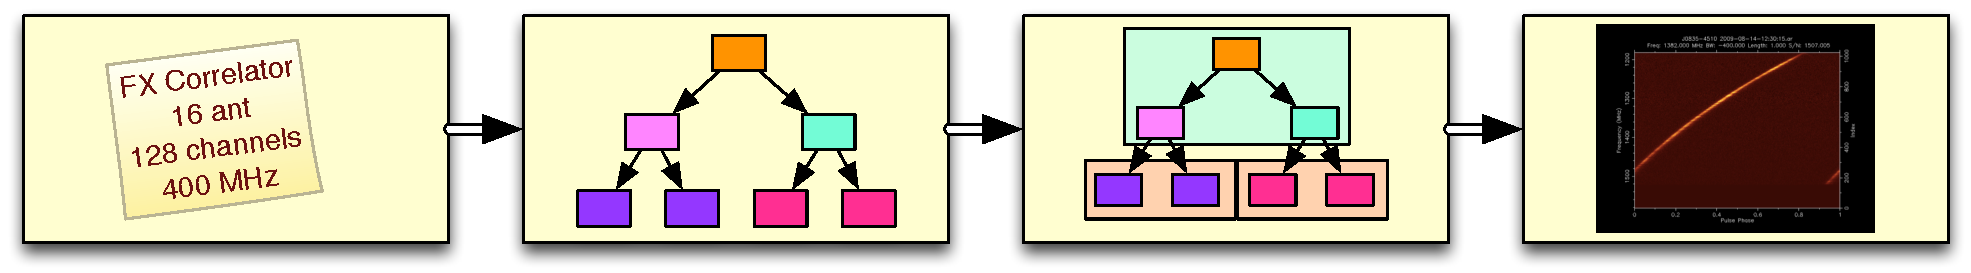
\includegraphics[width=1\textwidth]{Images/C4/toolflow_horizontal.pdf}
  \caption{TODO Toolflow}
  \label{fig: C4/toolflow_horizontal.pdf}
\end{figure}

These goals are achieved through a four stage toolflow. The rest of the chapter will describe each stage of the toolflow in more detail and explain how they are designed to meet the needs of these different users. 





\section{Instrument Definition} \label{High Level Toolflow:Instrument Definition}

%TODO: Add tool name
\begin{figure}[ht!]
  \centering
    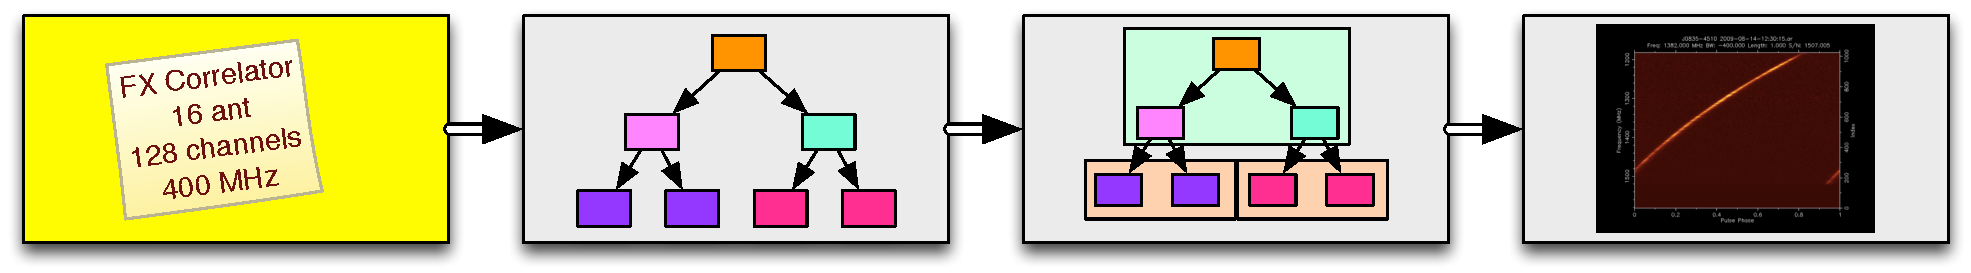
\includegraphics[width=1\textwidth]{Images/C4/toolflow_horizontal_s1.pdf}
  \caption{TODO Toolflow}
  \label{fig: C4/toolflow_horizontal_s1.pdf}
\end{figure}

%Describe instrument using parameters an astronomer can understand
%Small number of predefined instrument types
%Need to input
%Instrument type (predefined patterns)
%Total Bandwidth
%Array size (n)
%Etc
%Generates a dataflow representation
At the first step in the toolflow, the user must describe the instrument using high level parameters. 
These parameters should all 

%\begin{wrapfigure}[18]{l}{0.37\textwidth}
%  \centering
%     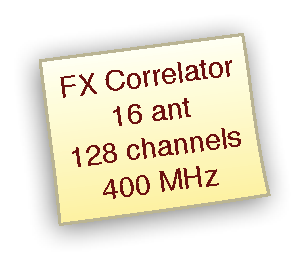
\includegraphics[width=0.2\textwidth]{Images/C4/instrument_description.pdf}
%  \caption{Example instrument description}
%  \label{fig:C4/instrument_description.pdf}
%\end{wrapfigure}


\section{Dataflow Model} \label{High Level Toolflow:Dataflow Model}
%TODO: Add tool name
\begin{figure}[ht!]
  \centering
    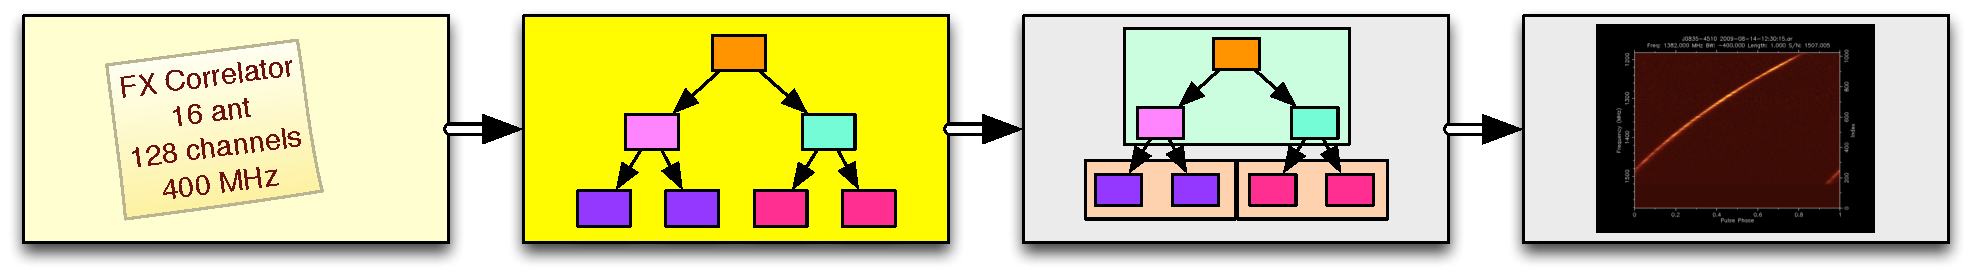
\includegraphics[width=1\textwidth]{Images/C4/toolflow_horizontal_s2.pdf}
  \caption{TODO Toolflow}
  \label{fig: C4/toolflow_horizontal_s2.pdf}
\end{figure}

\begin{figure}[ht!]
  \centering
    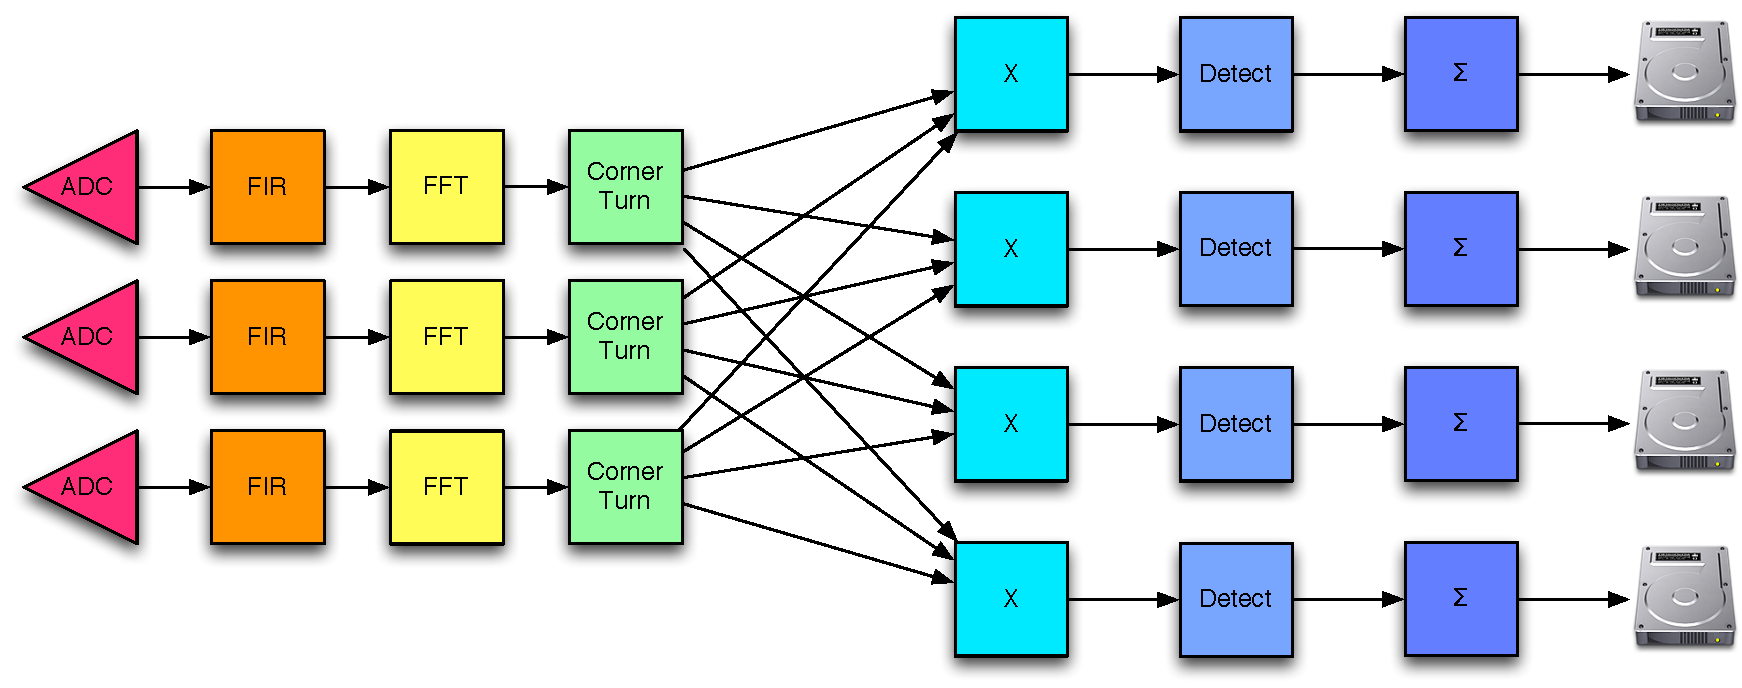
\includegraphics[width=1\textwidth]{Images/C4/fx_dataflow.pdf}
  \caption{Example FX Correlator Dataflow Model}
  \label{fig: C4/fx_dataflow.pdf}
\end{figure}

\subsection{Overview}

%Dataflow representation of instrument
%Define input/output connections
%Define input/output bandwidth
%Generates a series of blocks configured to talk to each other

\subsection{Computational Blocks}
%Collection of blocks necessary to solve most problems
%Can be parameterized
%Include a method to assess performance on each (supported) platform
%Performance model
%Benchmark
%Unit tests
%Uniform interconnect model
%Optimization: remove interconnect overhead for cores running on the same hardware

%Not certain this belongs here, possibly should go with the models?
%Before mapping, need to determine which blocks can be mapped to which platforms
%Synthesize/compile existing implementations to determine which platforms can support the spec
%Sanity check bandwidth requirements
%Test for acceptable noise tolerance in different implementations
%Known signals
%Test against arbitrary precision (exact) floating point implementation


\subsection{Connection Types}

Suppose we know we have 2 types of blocks: $A$, and $B$. 
Blocks of type $A$ must send their output to blocks of type $B$.
Now, we need to understand how blocks of type $A$ send data to blocks of type $B$.
This could happen in 2 ways, `one-to-one' and `all-to-all'. 

\begin{wrapfigure}[18]{l}{0.37\textwidth}
  \centering
    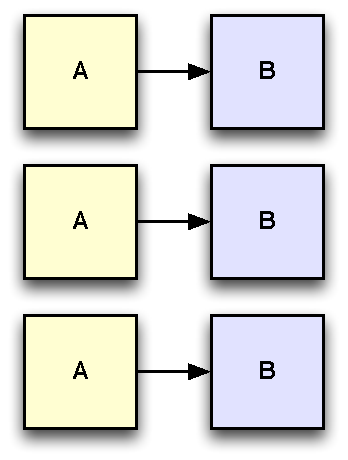
\includegraphics[width=0.35\textwidth]{Images/C5/one-to-one.pdf}
  \caption{TODO}
  \label{fig:one-to-one.pdf}
\end{wrapfigure}

A `one-to-one' connection is where every block of type $A$ communicates with exactly one block of type $B$, as shown in Figure \ref{fig:one-to-one.pdf}. 
With this type of connection, the number of blocks of type $A$ must be equal to the number of blocks of type $B$.
The F-engines in a FX correlator are a good example of this type of connection. 
The correlator has an F-engine for each antenna, each containing the same blocks linked in the same way. 
Within an F-engine, a PFB\_FIR filter must communicate with a single FFT.
In general, every PFB\_FIR within an F-engine, blocktype `A' must communicate with exactly one FFT, blocktype `B'. 



\begin{wrapfigure}[18]{r}{0.47\textwidth}
  \centering
    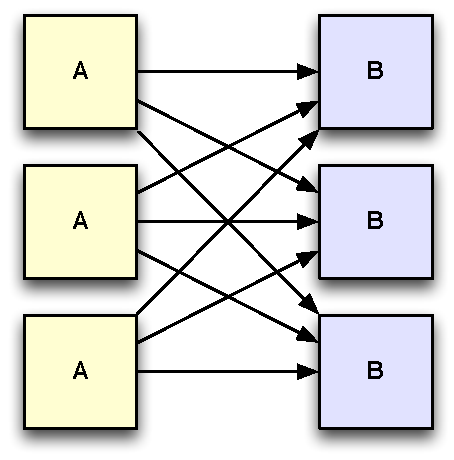
\includegraphics[width=0.45\textwidth]{Images/C5/all-to-all.pdf}
  \caption{TODO}
  \label{fig:all-to-all.pdf}
\end{wrapfigure}
      



An `all-to-all' connection occurs when every block of type $A$ must send some data to ever block of type $B$. 
Figure \ref{fig:all-to-all.pdf} shows what an all-to-all connection between 3 blocks of type $A$, and 3 blocks of type $B$ will look like. 
In this case, every block of type $A$ must send some data to every block of type $B$. 
For example, the type of connection between the per-antenna FFTs and the per-channel X-engines in an FX correlator would be `all-to-all'. 
Each X-engine needs a small amount of data from every F-engine to compute the cross-correlations from a single channel. 
In the `all-to-all' case, there is no reason for the number of sending nodes needs to be the same as the number of receiving nodes. 
%The n's do not get introduced until the ILP is defined
%This means that $n_{i,A}$ and $n_{i,B}$ do not have to be equal, and as long as the data can be distributed appropriately, there is no enforced relationship between the two variables. 




%TODO: make this an a,b figure
\begin{wrapfigure}{r}{0.47\textwidth}
  \centering
    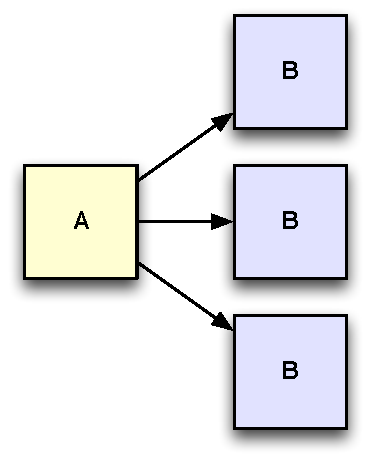
\includegraphics[width=0.4\textwidth]{Images/C5/one-to-all.pdf}
    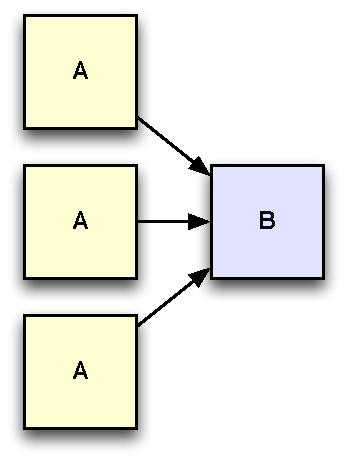
\includegraphics[width=0.4\textwidth]{Images/C5/all-to-one.pdf}
  \caption{TODO}
  \label{fig: one-to-all_vs_all-to-one}
\end{wrapfigure}



It might seem like there are two more possible types of connection, `one-to-all' and `all-to-one' .
A data flow with a `one-to-all' connection, shown in Figure x %TODO: fix reference, image
would have exactly one block of type $A$ that needs to send data to many blocks of type $B$. 
This is exemplified in the dataflow for a high-resolution spectrometer.
The coarse channelization is done in a single FFT block, which then needs to send the data to many other FFTs to do the fine channelization. 
The `all-to-one' connection shown in Figure x %TODO: fix ref
is there reverse of the `one-to-all' case. 
In this type of connection, there are many blocks of type $A$ and they all need to send data to a single instance of a block of type $B$. 
An example of this arises when some processing is done in a distributed manner but the instrument needs to record the final result in a central place. 
The $A$ blocks are responsible for the distributed processing, and then the $B$ block needs to collect the results and combine them.
%TODO: discuss scatter-gather?

It turns out, these are both special instances of the `all-to-all' connection. 
The `one-to-all' connection is simply an `all-to-all' where the number of $A$ blocks is fixed at 1.
Similarly, the `all-to-one' connection is also an `all-to-all' where the number of $B$ blocks is fixed at 1.
Because of this, there is no need to include or support these cases as unique connection types. 


While it may seem like additional link types exist like `all-to-some' or `one-to-some', this turns out to be impossible. 
Either a block of type $A$ cannot send its data to only some blocks of type $B$ because of the way blocktypes are defined.
Any block of the same type should be interchangeable with another block of the same type.
In an `all-to-some' connection, blocks of type $A$ would need to send data to $B_1$ but not send data to $B_2$.
But that connection patterns implies that the blocks $B_1$ and $B_2$ are \emph{not} interchangeable and therefore cannot have the same blocktype.


%TODO: This isn't implemented in the ILP
%TODO: Add correlator beamformer example. 
This does not preclude asymmetrical designs. 
Instead, asymmetry is supported by allowing blocks to define a list of blocktypes they must send data to or receive data from. 
The connection between any two blocktypes still must be described as above.

\subsection{Instrument Dataflows}
% Describe data flow for each instrument we are interested in implementing

\section{Mapping}
%TODO: Add tool name
\begin{figure}[ht!]
  \centering
    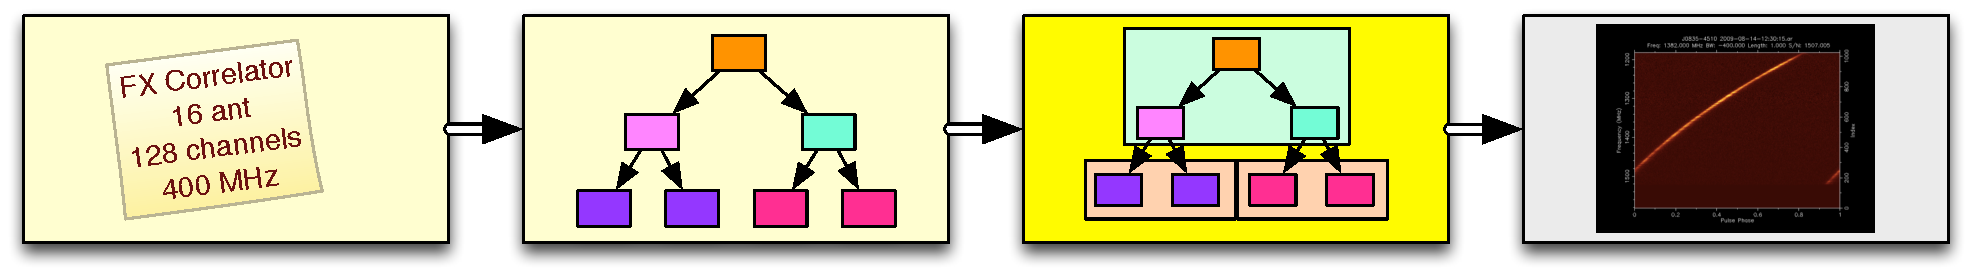
\includegraphics[width=1\textwidth]{Images/C4/toolflow_horizontal_s3.pdf}
  \caption{TODO Toolflow}
  \label{fig: C4/toolflow_horizontal_s3.pdf}
\end{figure}

\begin{figure}[ht!]
  \centering
    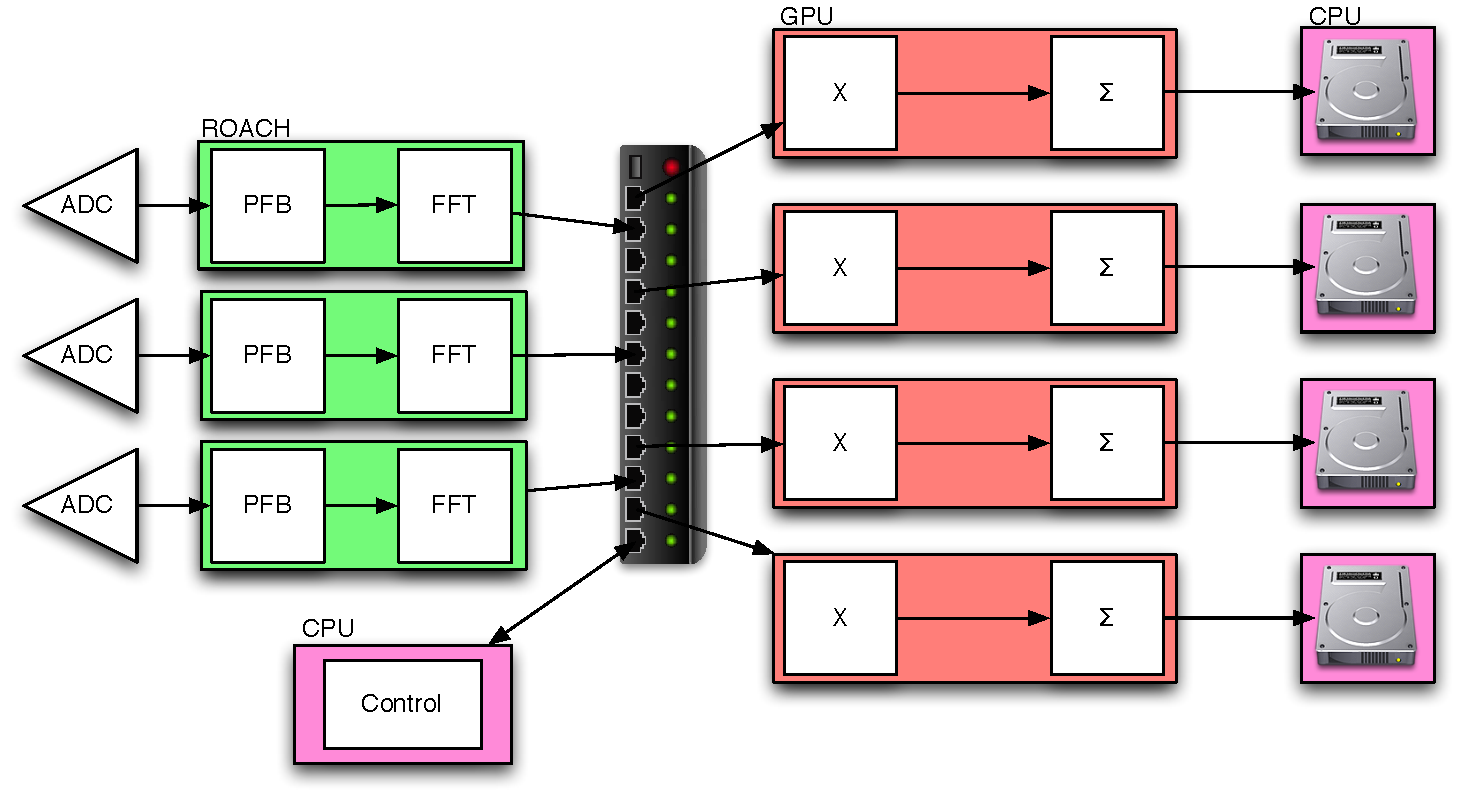
\includegraphics[width=\textwidth]{Images/C4/fx_mapped.pdf}
    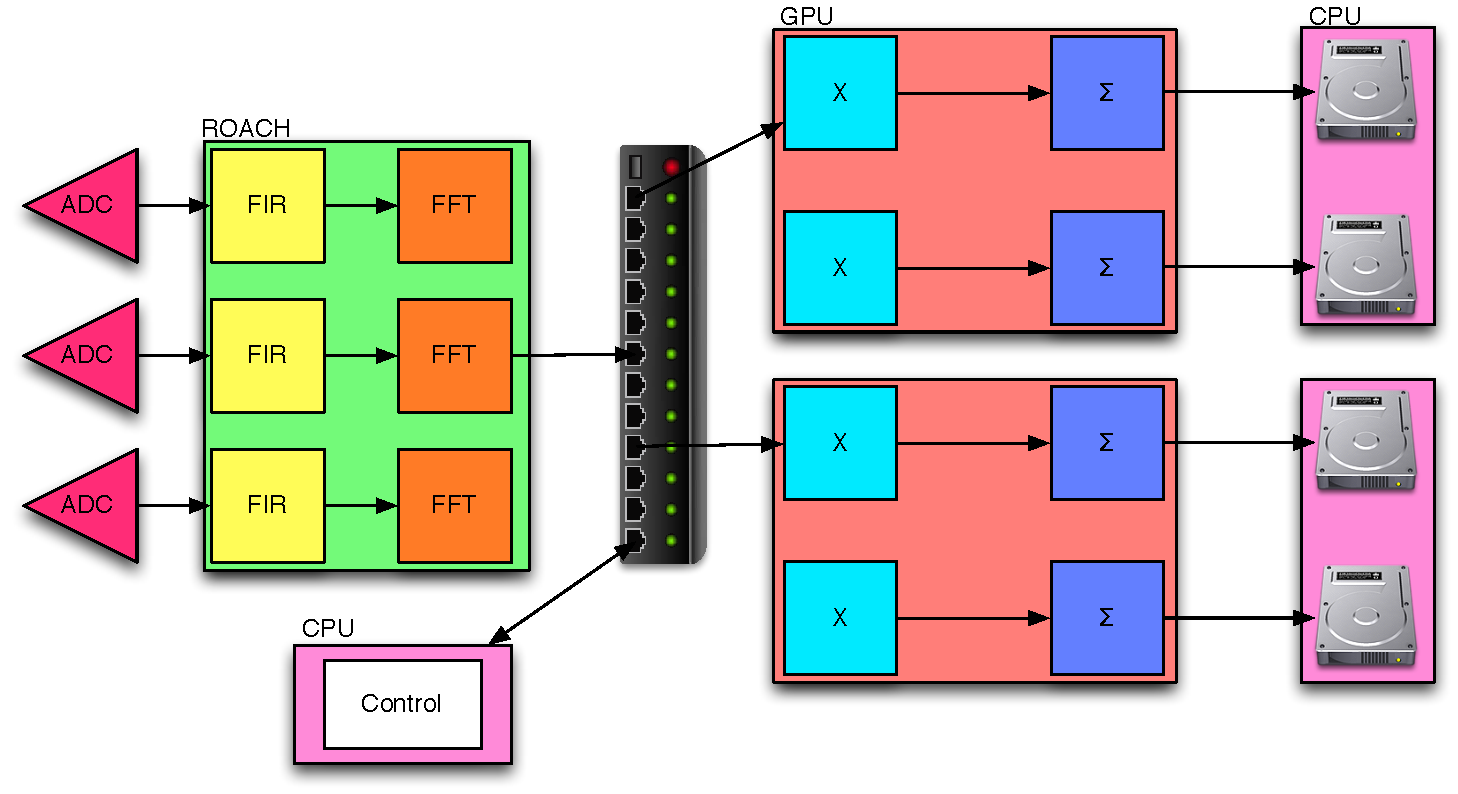
\includegraphics[width=\textwidth]{Images/C4/fx_mapped_alt.pdf}
  \caption{Two potential mappings for the FX Correlator}
  \label{fig: fft_vs_pfb_response}
\end{figure}

%TODO: think hard about this, we're not actually going to do this and it's optional
%This could be a good place to describe PASP, this is doable, we've shown it's possible
%Don't actually want to implement the entire thing but show feasibility
\section{Code Generation}
%TODO: Add tool name
\begin{figure}[ht!]
  \centering
    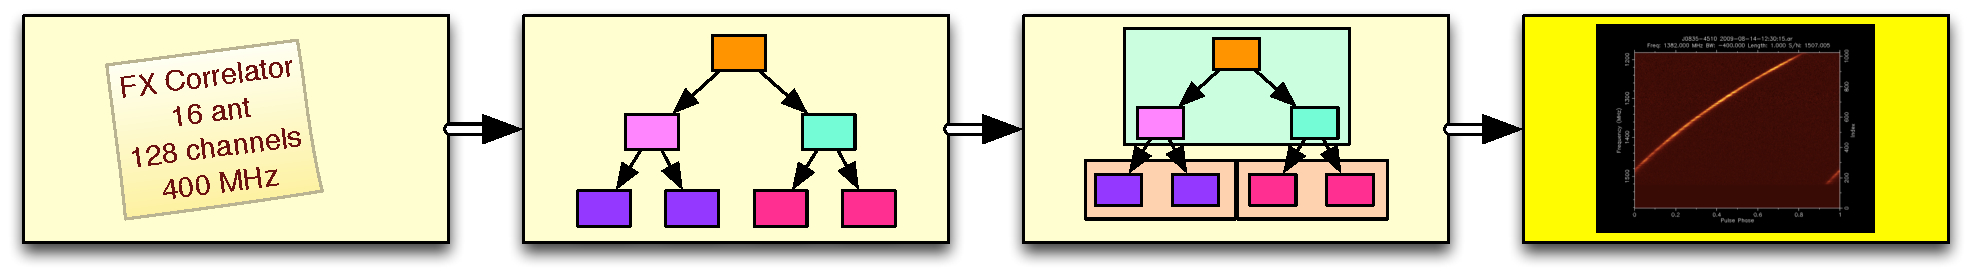
\includegraphics[width=1\textwidth]{Images/C4/toolflow_horizontal_s4.pdf}
  \caption{TODO Toolflow}
  \label{fig: C4/toolflow_horizontal_s4.pdf}
\end{figure}

%Use a mapped dataflow to stitch together blocks
%To generate code the blocks must have an implementation for the target platform (not necessary for mapping)
%Include an automatic test suite for each platform
%Block communication is standardized so they can be connected in arbitrary ways
\subsection{Packetized Astronomy Signal Processor}

This instrument has a wide variety of potential applications due to the flexibility of the server software. 
In this section, we describe a few specific applications than can make use of this package.

In the search for extraterrestrial intelligence (SETI), the ability to keep up with changes in technology allows searching instrumentation to stay on the leading edge of sensitivity. 
SETI aims to process the maximum bandwidth possible with very high resolution spectroscopy.
This instrument allows SETI projects to easily keep up with improvements on the telescope and increasing computational power.
An increase in detector bandwidth, improving the breadth of the search, can be processed simply recompiling the FPGA design and distributing the extra subbands to new servers. 
As computation improves, the instrument can be reconfigured to send more bandwidth to each computer, reducing the required cluster size, or improve the resolution of the instrument by doing a larger FFT on the server.

This design also has applications in pulsar science. 
The fast channelization on the FPGA with no data reduction makes it an ideal pulsar spectrometer, since no information is lost before sending the data to the servers.
GPUs provide a good platform for pulsar processing algorithms such as coherent dedispersion \cite{Ransom:2009wz}, which can easily be used as the processing function for the server software distributed in our package. 
Similar to SETI instruments, pulsar instruments designed using this package can also keep up with improvements in technology with a simple recompile.

Figure \ref{fig: pasp_fpga_arch} gives an overview of the dataflow through the FPGA.
The FPGA interfaces to a single ADC board that simultaneously digitizes 2 signals. 
Each signal can be sampled at a maximum rate of 1Msps.
The samples are sent into a polyphase filter bank (PFB), consisting of an FIR filter and an FFT, which breaks up the entire bandwidth sampled by the ADC into smaller subbands.
After dividing up the subbands, each band is rescaled. 
This step allows us to compensate for the shape of the analog filter feeding data into the ADC. 
After rescaling, the FPGA forms packets where each packet contains data from a single subband. %TODO fix
The packets are sent out over CX4 ports to a 10 gigabit Ethernet switch.

\begin{figure}[ht!]
  \centering
    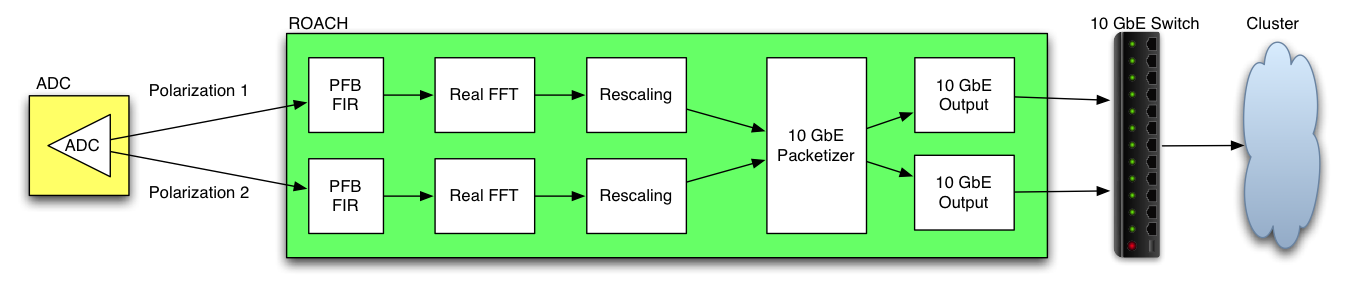
\includegraphics[width=1\textwidth]{Images/C4/pasp_fpga_arch.png}
  \caption{PASP Dataflow}
  \label{fig: pasp_fpga_arch}
\end{figure}

PASP uses a PFB to split up the subbands. Figure \ref{fig: fft_vs_pfb_response} shows a comparison between the FFT and PFB response. 
The FFT response (on the left) has a lot of spectral leakage while the PFB (on the right) has a much sharper filter shape and a better frequency response. 
The superior frequency response led us to use a PFB rather than an FFT to extract subbands, despite the additional FPGA resources required by the FIR filter before the FFT.

\begin{figure}[ht!]
  \centering
    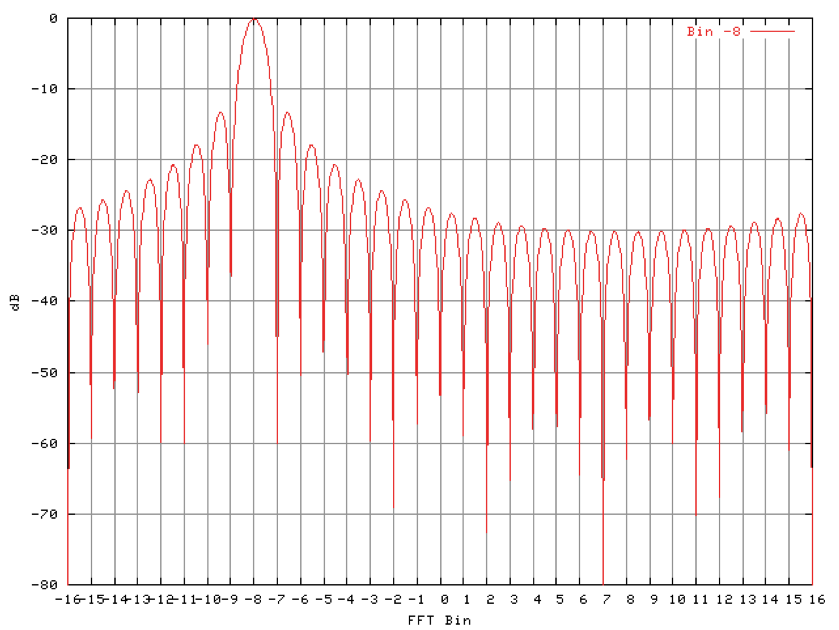
\includegraphics[width=0.48\textwidth]{Images/C4/fft_response.png}
    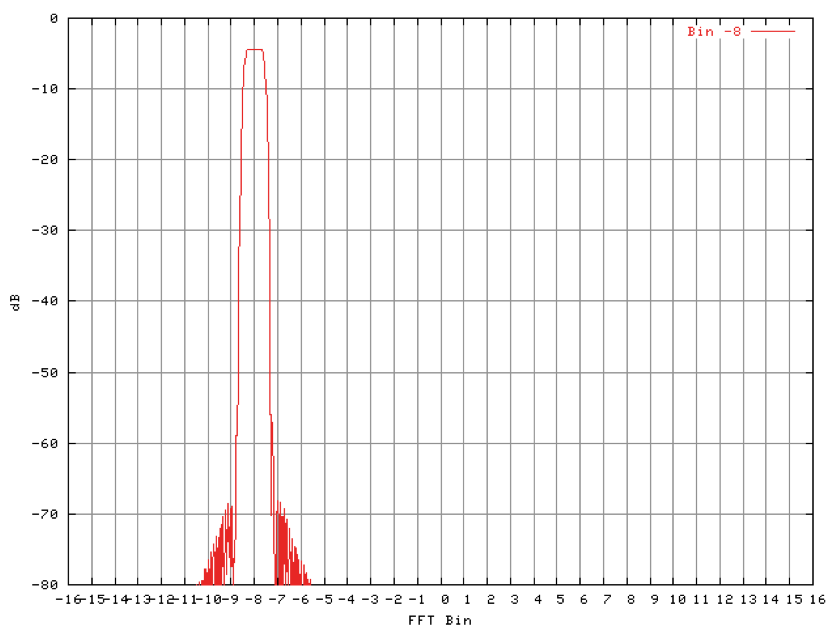
\includegraphics[width=0.48\textwidth]{Images/C4/pfb_response.png}
  \caption{A comparison of FFT and PFB response}
  \label{fig: fft_vs_pfb_response}
\end{figure}

PASP is designed for flexibility. 
Building on the CASPER goal to automate the design of commonly used signal processing elements such as FFTs and digital downconverters, PASP automatically designs an entire FPGA instrument using only a few parameters.
The user can input the desired number of subbands, CPU/GPU cluster size, and packet size and a new design is automatically generated in Simulink.  

\subsection{Heterogeneous Radio SETI Spectrometer}
We have developed a software package to automatically generate spectrometers with minimal user input.

We have automated this design, creating a parameterized spectrometer that only requires a recompile to implement a change in specification.
This spectrometer combines FPGAs and GPUs, doing coarse channelization on the FPGA and sending each subband to the GPUs for further processing.
The server software is designed for flexibility, allowing astronomers to easily modify the processing algorithm run on the GPU and customize the instrument to fit their science goals.

The software package includes an FPGA design and server software to do spectroscopy, as well as server benchmarks used to determine an optimal instrument configuration.
%The benchmarks measure maximum amount of data the servers can process, determining the optimal configuration for the instrument.
Both the FPGA and server software are parameterized, allowing for rapid deployment of a working spectrometer that is configured to take full advantage of available computing resources.
%Our general purpose approach allows for the rapid development of new instruments.
We implement the instrument on a heterogeneous cluster consisting of both FPGAs and GPUs to take advantage of the benefits provided by both platforms.
FPGAs provide high bandwidth processing but can be cumbersome to program.
GPUs can't handle the same bandwidths as FPGAs but they are easier to program. 
The CUDA language, for example, is a C-like language that can be used to develop software for many GPUs.
The high level parameters in this package allow us to use FPGAs while abstracting away implementation details specific to the FPGA.
To give the user control over their data processing algorithm, an application specific GPU program can be written and easily interfaced with the existing receive software in the package.


The instruments generated with this package use a heterogeneous design, allowing us to benefit from the strengths of FPGAs and GPUs. 
The FPGA board is able to sample and process very high bandwidths that a single CPU or GPU would not be able to manage; 
once the FPGA has split up the band the GPU provides a platform that is easier than an FPGA to program but still provides high compute power. 
A design called the Packetized Astronomy Signal Processor, or PASP, is run on the FPGA.
PASP splits up the large band into smaller bands that can be processed using off the shelf servers.
The subbands are put into packets on the FPGA and sent over a 10 gigabit Ethernet switch to a cluster of servers.
The servers receive the data from the switch and process it using spectroscopy software provided in the software package or special purpose application software written by the user and linked into the provided packet processing infrastructure.

Figure \ref{fig:spec_highlevel} shows a high level view of a spectrometer that could be designed with this package. 
In this example, a ROACH board divides the input band into 64 subbands and sends them out to a 16 server cluster.
An ADC is used to digitize data from the telescope and connects to the ROACH board via Z-DOK connectors. 
The digitized data is split into 64 subbands and sent through a 10 gigabit Ethernet switch.
Each server in the cluster receives and processes 4 subbands.

\begin{figure}[ht!]
  \centering
     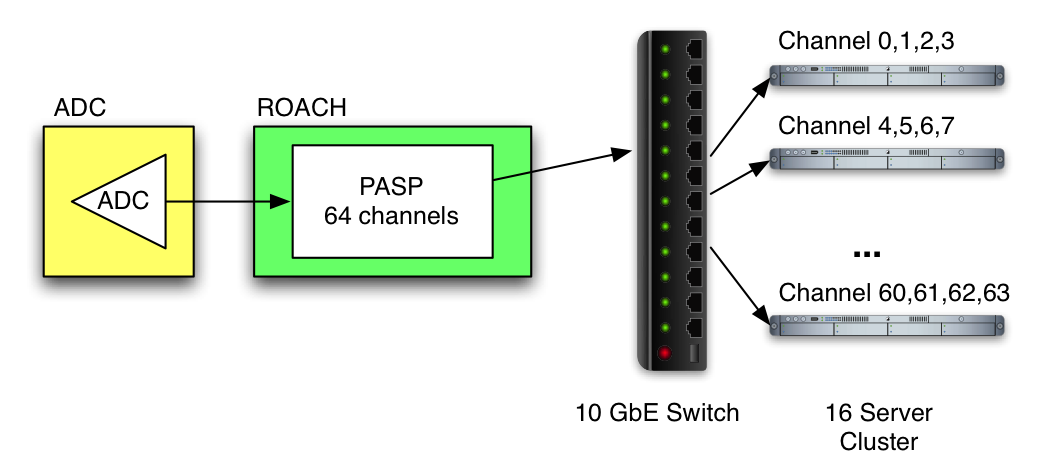
\includegraphics[width=1\textwidth]{Images/C4/spec_highlevel.png}
  \caption{Example high level instrument architecture}
  \label{fig:spec_highlevel}
\end{figure}

\subsubsection{Server Software}
Our package includes spectroscopy software that interfaces with the PASP design.
This software receives data over an Ethernet port and transfers it from the CPU to the GPU. 
The GPU runs an FFT and then sends the data back to the CPU to be recorded.
The GPU software, like the GPU benchmark, uses the CUFFT library to run FFT. 
The FFT size depends on the desired resolution for a specific application and an efficient batch size can be determined by running the FFT benchmark to find the best batch size for the given FFT size.

The server software was designed so other applications could easily be implemented on the GPU without altering or rewriting the receive code that interprets the packet headers and transfers data to the GPU.
Once the data is on the GPU, the software calls a process function and passes it a pointer to the GPU data.
An initialization function is called before the data processing begins to do any setup needed by the processing function, and an corresponding destroy function cleans up once the processing is complete.
In the spectroscopy software included in the package, the initialization function creates the FFT plan, the processing function calls CUFFT, and the destroy function deletes the FFT plan.
Modifying the application run on the GPU simply requires a redefinition of these three functions.
Using this interface, we successfully replaced the CUFFT processing with software developed for SETI searches designed by Kondo et al. \cite{Kondo:2010uk}.

In this paper, we describe a radio astronomy instrument that is easily reconfigured to suit a variety of applications.
Figure \ref{fig: universal_arch} shows how this style of instrument design can be extended to a heterogeneous cluster running multiple processing algorithms at the same time.
All of these algorithms require the data to be broken up into subbands before it can be processed by the server which can be done on the same FPGA. 
Using multicast packets, multiple servers can subscribe to the same subbands generated on by PASP and process them in different ways. 


This style of instrument design greatly accelerates time to science for many projects.
Separating the implementation of the instrument from the hardware specification has created a design that works well for a variety of computational resources and applications.
As resources improve, the instrument can improve along with them, providing the opportunity to do new science that wasn't possible before.



